\chapter{Zbieranie i przetwarzanie danych z czujników}

\section*{Raspberry Pi}

Wszystkie zestawy zbudowaliśmy w oparciu o Raspberry Pi 3 v1.2. Zdecydowaliśmy się na to rozwiązanie, ponieważ bazuje on na dystrybucji Linuxa, posiada opowiednie interfejsy i złącza a także zintegrowany moduł WiFi. Minusem w stosunku do konkurencyjnego Arduino jest brak wejść analogowych. Problem rozwiązano dodając zewnętrzny przetwornik A/C.
\paragraph{Specyfikacja Raspberry Pi 3:}
\begin{itemize} 
\item Procesor 1.2 GHz
\item Liczba rdzeni 4. Quad Core
\item Pamięć RAM 1 GB
\item Pamięć Karta microSD
\item 40 GPIO
\end{itemize}
\begin{figure}[h]
	\centering
	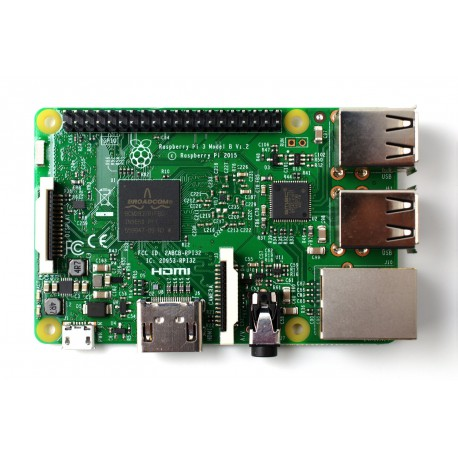
\includegraphics[width=6cm]{raspberry.jpg}
	\caption{Raspberry Pi 3}
\end{figure}
Aby prawidłowo zainstalować oprogramowanie The Guard na dowolnym urządzeniu Raspberry Pi 3 należy wykonać poniższe czynności w terminalu:
\begin{enumerate} 
\item sudo apt-get install libx264-dev
\item cd /usr/src
\item git clone git://source.ffmpeg.org/ffmpeg.git
\item sudo ./configure --arch=armel --target-os=linux --enable-gpl --enable-libx264 --enable-nonfree
\item sudo make
\item sudo install
\item sudo nano /boot/config.txt
\item dopisać w pliku Dtoverlay=w1-gpio i Gpiopin=4
\item pip intall wiringpi
\item sudo pip install spidev
\item pip install pyrebase
\end{enumerate}
Następnym krokiem jest włączenie odpowiednich interfejsów w panelu konfiguracyjnym. Należy zmienić ustawienia zgodnie z poniższym schematem:

\begin{figure}[h]
	\centering
	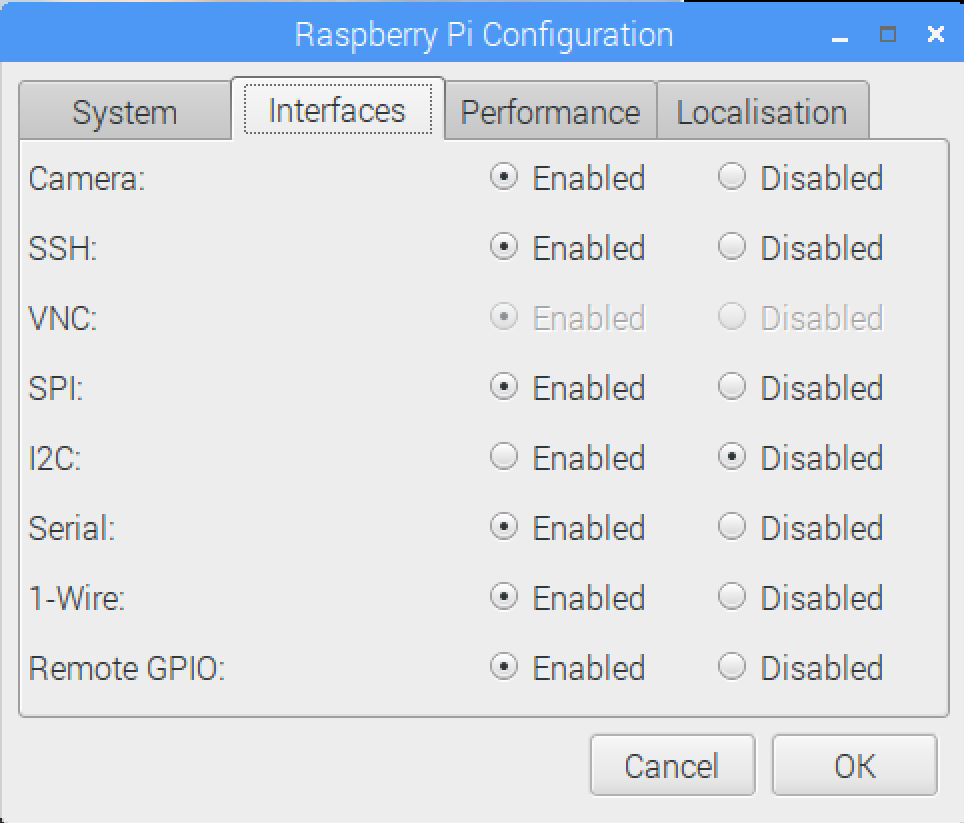
\includegraphics[width=6cm]{RSettings}
	\caption{Ustawienia}
\end{figure}

W kodzie używamy biblioteki wiringpi do odczytu danych z układów cyfrowych. Należy zaznaczyć, że numeracja fizycznych pinów i numeracja pinów w bibliotece wiringPi jest różna i nie zawiera wszystkich dostępnych pinów na urządzeniu. 

\begin{figure}[h]
  \centering
  \begin{minipage}[b]{0.4\textwidth}
    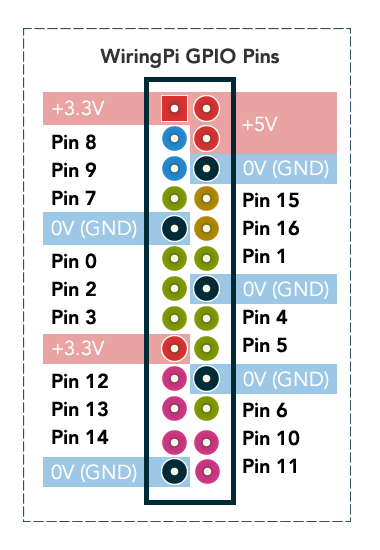
\includegraphics[width=\textwidth]{wiringpi.png}
    \caption{WiringPi}
  \end{minipage}
  \hfill
  \begin{minipage}[b]{0.4\textwidth}
    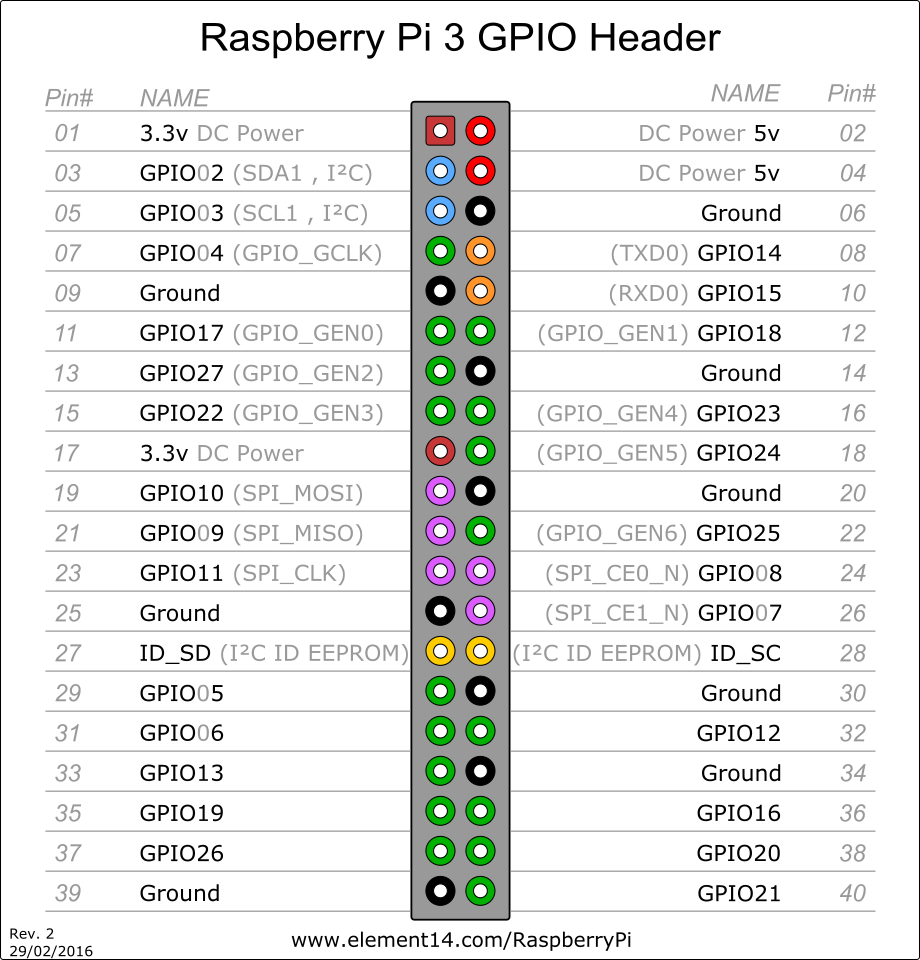
\includegraphics[width=\textwidth]{gpio.png}
    \caption{GPIO}
  \end{minipage}
\end{figure}

Oprogramowanie zainstalowane na Raspberry Pi odpowiedzialne jest za ciągłe monitorowanie stanów i danych z czujników pomiarowych. Po podłączeniu układu do zasilania oprogramowanie jest uruchamiane automatycznie. Pierwszą czynnością jaką wykonuje Raspberry jest wysłanie swojego numery seryjnego do bazy danych Firebase. Cały proces jest w pełni zautomatyzowany. Dzięki temu użytkownicy od razu mogą dodać urządzenie i monitorować dane z czujników na aplikacjach klienckich. Dodawanie urządzenia następuje poprzez wprowadzenie w aplikacji numery seryjnego urządzenia, które chcę dołączyć do mojego konta użytkownika.


\section*{Czujniki}

Każdy zestaw składa się z 5 czujników analogowo cyfrowych,  jednej kamery i jednego przetwornika AC. 
\paragraph{a) Specyfikacja MQ-9 - czujnik tlenku węgla:}
\begin{itemize} 
\item Zasilanie: 5 V
\item Pobór prądu: 150 mA
\item Temperatura pracy: od -10 do 50 \textdegree{}C
\item Wyjścia: analogowe oraz cyfrowe
\end{itemize}

\paragraph{b) Specyfikacja MQ-2 - czujnik LPG i dymu:}
\begin{itemize} 
\item Zasilanie: 5 V
\item Pobór prądu: 150 mA
\item Temperatura pracy: od -10 do 50 \textdegree{}C
\item Wyjścia: analogowe oraz cyfrowe
\end{itemize}

\paragraph{c) Specyfikacja czujnika wykrywania płomieni:}
\begin{itemize} 
\item Zasilanie: 3.3 V
\item Zakres wykrywanej fali: 760 do 1100nm
\item Kąt detekcji: od 0 do 60 stopni
\item Temperatura pracy: od -25 do 85 \textdegree{}C
\end{itemize}

\paragraph{d) Specyfikacja DS18B20 - czujnik temperatury:}
\begin{itemize} 
\item Zasilanie: 3.3 V
\item Zakres pomiarowy: od -55 do 125 \textdegree{}C
\end{itemize}

\paragraph{e) Kamera:}
\begin{itemize} 
\item Wykorzystano moduł kamery Raspberry Pi element14
\item Kamera 5MP - wspierająca nagrywanie 30 klatek na sekundę w rozdzielczości Full HD
\end{itemize}

\paragraph{f) Specyfikacja MCP3008 - przetwornik A/C:}
\begin{itemize} 
\item Zasilanie: od 2.7V do 5.5V
\item Pobór prądu: 0.5 mA
\item Interfejs komunikacyjny: SPI
\item Liczba kanałów: 8
\item Rozdzielczość: 10bit
\item Czas konwersji: 10us
\end{itemize}

\begin{figure}[h]
	\centering
	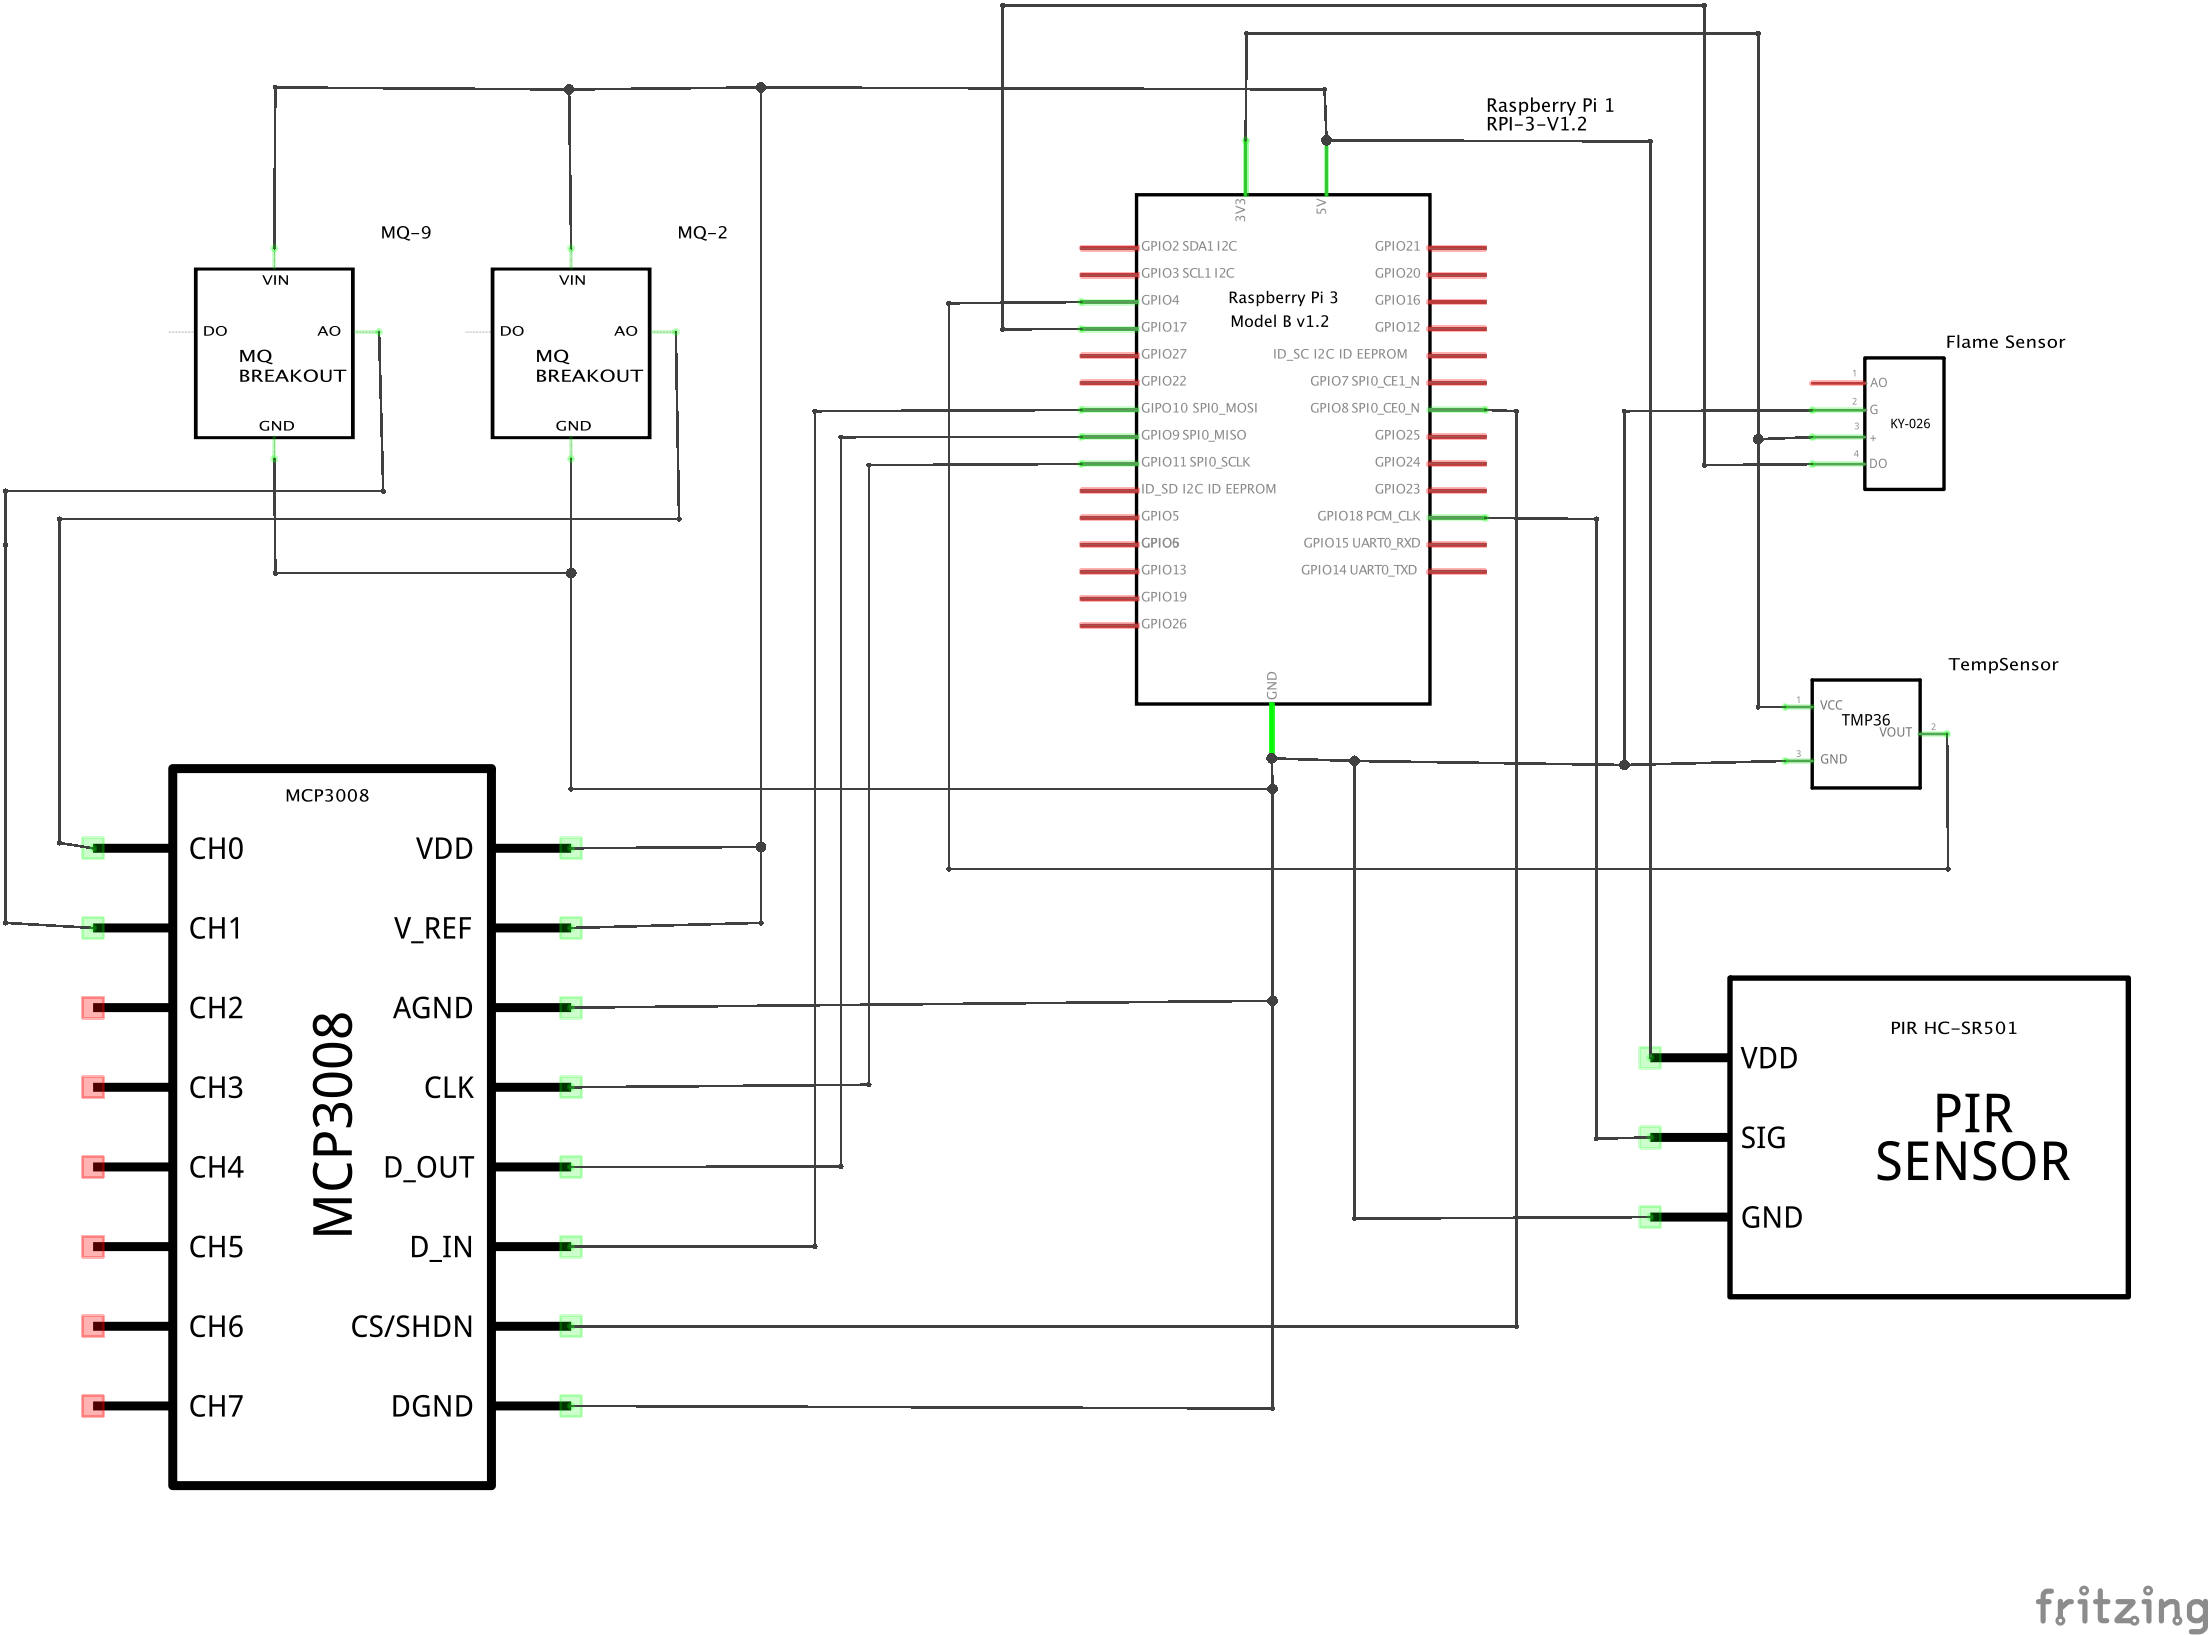
\includegraphics[width=15cm]{GuardSchem}
	\caption{Schemat układu The Guard}
\end{figure}

Niestety żaden model Raspberry nie posiada wbudowanego przetwornika analogowo cyfrowego dlatego konieczne było użycie układu zewnętrzenego. Wybraliśmy przetwornik MCP3008 ze względu na jego nisko koszt i interfejs SPI, który jest wspierany przez Raspberry Pi.
MCP3008 to 10-bitowy przetwornik analogowy cyfrowy. Zasilany jest napięciem 5V, napięcie VRef = 5V.  Skoro jest to przetwornik 10-bitowy jest w stanie wykryć 1024 stanów. Wykrywana przez niego minimalna różnica napięć na wejściu wynosi 
\begin{equation}
1 * 5V / 1024 = 4.88mV
\end{equation}
Posiada 8 kanałów jednak w projekcie wykorzystano tylko 2 – do podłączenia czujników MQ-9 i MQ-2.

\paragraph{Interfejs SPI:}
\begin{figure}[h]
	\centering
	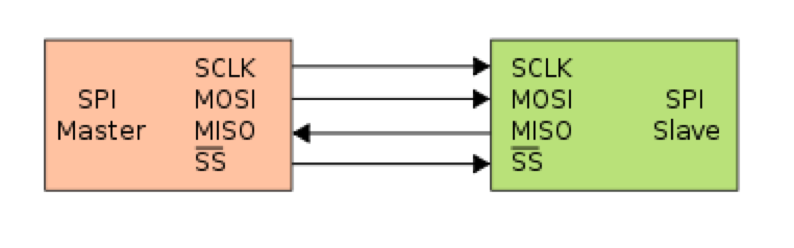
\includegraphics[width=6cm]{SPI.png}
	\caption{Interfejs SPI}
\end{figure}
SPI jest to interfejs synchroniczny. Może być do niego podłączone wiele urządzeń typu slave, jednak tylko z jednym urządzeniem Master, który generuje zegar. Master poprzez linię SS wybiera urządzenie z którym chce się komunikować.  \\
Interfejs ten zawiera jeszcze 3 linie:
\begin{enumerate} 
\item MOSI (ang. Master Output Slave Input): \\
Poprzez tę linię wysyłane są dane z Raspberry Pi do przetwornika analogowo cyfrowego MCP3008.
\item MISO (ang. Master Input Slave Output):\\
Poprzez tę linię wysyłane są dane z przetwornika AC do układu Master czyli w naszym przypadku Raspberry Pi 3
\item SCLK (ang. Serial CLocK) :\\
Ta linia wykorzystywana jest do przesłania zegara wygenerowanego z Rapberry Pi 3
\end{enumerate}
Do komunikacji poprzez ten interfejs wykorzystano bibliotekę spiDev. \\


Każdy układ monitoruje wskaźniki pomiarowe z czujników analogowych i cyfrowych. W przypadku wykrycia wskazań, które w znaczący sposób odbiegają od normy informuje właściciela o zagrożeniu. Informacja ta wysyłana jest do wszystkich urządzeń, które posiada właściciel.  Analizując dane z czujników analogowych w czytym powietrzu, które wynoszą wtedy odpowiednio:\\
Czujnik MQ-9: 0.15 – 0.2\\
Czujnik MQ-2: 0.05 – 0.15\\
Przyjęto, że granicą wysłania notyfikacji do urządzeń użytkownika jest przekroczenie progu 0.3. Wartości te to znormalizowane dane z układu przetwornika AC, który jak już wcześniej wspomniałem wykrywa 1024 stany. Odczytywane wartości bezpośrednio na wyjściu cyfrowym przetwornika MCP3008 dla czujnika MQ-9 w czystym powietrzu to około 170. Stąd 170/1024 = 0.166. Wysłanie notyfikacji wiąże się z otrzymaniem wartości min. 308 bezpośrednio na wyjściu cyfrowym.
Reszta to czujniki cyfrowe, które informują m.in. o wykryciu ognia i wykryciu ruchu. W przypadku detekcji zagrożenia wysyłają one na wyjście stan niski i utrzymują go przez kilka sekund. W kodzie jednak wykonujemy instrukcje negacji tak, aby stan wysoki informował o niebezpieczeństwie a stan nisko reprezentował jego brak. Na obu czujnikach znajduje się potencjometr, za pomocą którego dowolnie można ustawiać czułość czujnika.
Bezpośredni odczyt danych z czujników następuje nieprzerwanie co 2 sekundy. Nie należy obawiać się, że czujnik ruchu nie wykryje zagrożenia gdyż nie zostanie odczytany w poprawnym czasie, ponieważ utrzymuje on stan wysoki przez 5 sekund po wykryciu ruchu.
Oprogramowanie oprócz monitorowania danych z czujników wysyła je także do bazy danych Firebase. Dzięki temu mamy podgląd wszystkich danych z każdego z pomieszczeń w czasie rzeczywistym. Dodatkowo w przypadku wykrycia zagrożenia czyli przekroczeniu progu o którym mowa wyżej wysyłamy push notyfikacje do wszystkich urządzeń użytkownika i zapisujemy wysłaną notyfikację w bazie danych Django. Dzięki zapisywaniu danych jesteśmy w stanie odtworzyć całą historię wydarzeń w systemie.
Aby zapewnić wydajny i pewny system bezpieczeństwa przy otrzymaniu wysokich wartości na czujnikach i wysłaniu notyfikacji zapisujemy timestamp zdarzenia. Dzięki temu nie ma możliwości zasypania właściciela miliardem informacji gdyż każda kolejna notyfikacja zostanie wysłana po min. 10 min od poprzedniej przy założeniu, że nadal stan na czujniku jest wysoki.
W przypadku iOS, Apple monitoruje ilość wysłanych push notyfikacji do konkretnego urządzenia. Kiedy ich ilość będzie wysoka zostanie to potraktowane jako spam i zostanie nałożona blokada aby chronić użytkownika przed niechcianymi informacjami. W naszym przypadku nie możemy do tego dopuścić a poprzez mechanizm timestampów zapobiegamy nałożeniu blokady.




















\section*{Obsługa wideo}

Opis procesu, opis Nginxa, opis RTMP i HLS